\documentclass[tikz, border=20pt]{standalone}
\usepackage{amsmath, amssymb}
\usetikzlibrary{positioning, arrows.meta, shapes.geometric, calc, shadows.blur}

\begin{document}
	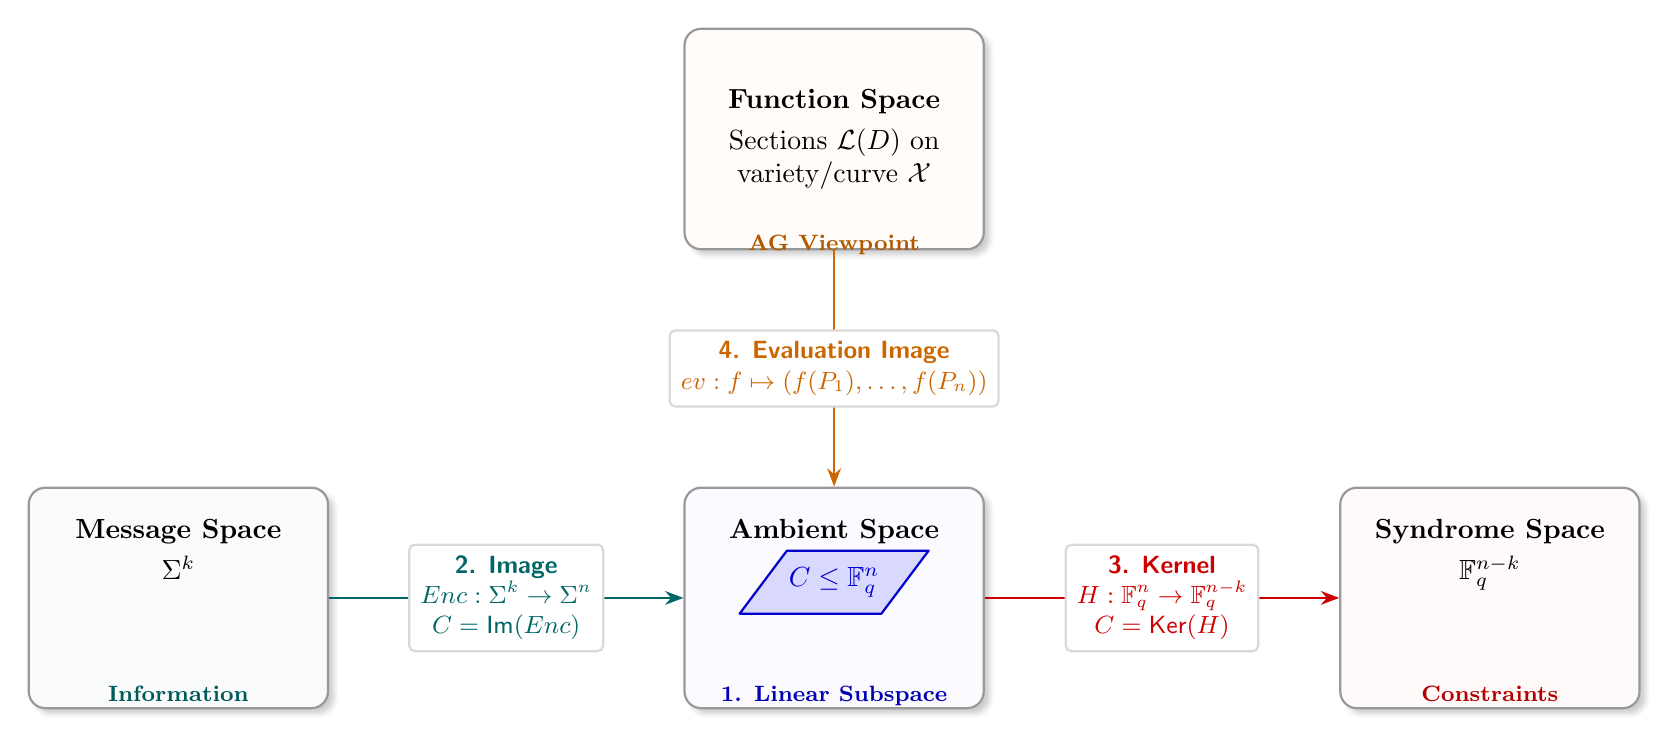
\begin{tikzpicture}[
		>=Stealth,
		% Styles for the domain boxes
		space/.style={
			draw=gray!80, thick, fill=white, rounded corners=6pt,
			minimum width=3.8cm, minimum height=2.8cm, align=center,
			blur shadow={shadow blur steps=5, shadow opacity=20, shadow yshift=-2pt}
		},
		% Style for the arrow labels
		arrow_label/.style={
			midway, align=center, font=\small\sffamily, fill=white, inner sep=4pt,
			draw=gray!30, rounded corners=2pt
		}
		]
		
		% Custom finite field macro
		\newcommand{\F}{\mathbb{F}}
		
		% ==========================================
		% 1. THE CENTER: Ambient Space & Subspace
		% ==========================================
		\node[space, fill=blue!2] (ambient) {
			\textbf{Ambient Space} \\[0.1cm] $\Sigma^n = \F_q^n$ \\[0.8cm]
		};
		
		% Draw the 1st bullet point: the linear subspace C
		\draw[thick, fill=blue!15, draw=blue!80!black, join=round]
		($(ambient.center) + (-1.2,-0.2)$) -- ($(ambient.center) + (0.6,-0.2)$) -- 
		($(ambient.center) + (1.2,0.6)$) -- ($(ambient.center) + (-0.6,0.6)$) -- cycle;
		\node[font=\bfseries, text=blue!80!black] at ($(ambient.center) + (0, 0.2)$) {$C \leq \F_q^n$};
		
		% Bullet 1 Label
		\node[font=\footnotesize\bfseries, text=blue!70!black, below=1cm of ambient.center] {1. Linear Subspace};
		
		% ==========================================
		% 2. THE LEFT: Generative / Image View
		% ==========================================
		\node[space, left=4.5cm of ambient, fill=teal!2] (message) {
			\textbf{Message Space} \\[0.1cm] $\Sigma^k$ \\[0.8cm]
		};
		\node[font=\footnotesize\bfseries, text=teal!70!black, below=1cm of message.center] {Information};
		
		% Arrow for Bullet 2
		\draw[->, thick, teal!80!black] (message.east) -- (ambient.west)
		node[arrow_label] {\textbf{2. Image} \\ $Enc: \Sigma^k \to \Sigma^n$ \\ $C = \text{Im}(Enc)$};
		
		% ==========================================
		% 3. THE RIGHT: Checking / Kernel View
		% ==========================================
		\node[space, right=4.5cm of ambient, fill=red!2] (syndrome) {
			\textbf{Syndrome Space} \\[0.1cm] $\F_q^{n-k}$ \\[0.8cm]
		};
		\node[font=\footnotesize\bfseries, text=red!70!black, below=1cm of syndrome.center] {Constraints};
		
		% Arrow for Bullet 3
		\draw[->, thick, red!80!black] (ambient.east) -- (syndrome.west)
		node[arrow_label] {\textbf{3. Kernel} \\ $H: \F_q^n \to \F_q^{n-k}$ \\ $C = \text{Ker}(H)$};
		
		% ==========================================
		% 4. THE TOP: Algebraic Geometry View
		% ==========================================
		\node[space, above=3cm of ambient, fill=orange!2] (ag) {
			\textbf{Function Space} \\[0.1cm] Sections $\mathcal{L}(D)$ on \\ variety/curve $\mathcal{X}$
		};
		\node[font=\footnotesize\bfseries, text=orange!70!black, below=1.1cm of ag.center] {AG Viewpoint};
		
		% Arrow for Bullet 4
		\draw[->, thick, orange!80!black] (ag.south) -- (ambient.north)
		node[arrow_label] {\textbf{4. Evaluation Image} \\ $ev: f \mapsto (f(P_1), \dots, f(P_n))$};
		
	\end{tikzpicture}
\end{document}